\section{Prezentacja wyników pracy - 01.06.2023r.}
    Dnia 01.06.2023r. dokonano następujących postępów:
    \begin{itemize}
        \item zaprojektowano interfejs widoku ,,Wilgotność'' (Rysunek \ref{fig: hum tab}),
        \item zaprojektowano interfejs widoku ,,Wypełnienie''(Rysunek \ref{fig: vol tab}),
        \item połączono sloty odpowiedzialne za aktualizacje właściwych im danych dotyczących elementów
        interfejsu, takich jak:
            \begin{itemize}
                \item graficzna i tekstowa prezentacja wilgotność i wypełnienia silosu (widoki ,, Wilgotność'' i ,,Wypełnienie''),
                \item Prezentacja informacji o alarmach (widoki „Wilgotność” i „Wypełnienie”),
            \end{itemize}
        \item zaimplementowano obsługę małej bazy danych pracującej w systemie SQLite - stworzono klasę reprezentującą bazę danych, oferującą
        prosty interface pozwalający na zapis i odczyt danych.
        \item zaprojektowano interfejs widoku ,,Dane Historyczne''(Rysunek \ref{fig: hist data tab}):
        \begin{itemize}
            \item na interfejsie umieszczono elementy pozwalające wybrać dane do wizualizacji i obiekt reprezentujący wykres,
            \item dokonano odpowiednich połączeń sygnałów z elementów Ui ze slotami odpowiedzialnymi za prace backendową, w tym obsługę pracy z bazą danych,
        \end{itemize}
        \item napisano tłumaczenie aplikacji na język angielski, użytkownik ma możliwość wyboru języka (Rysunek \ref{fig: ang}).
    \end{itemize}
    \subsection{Aplikacja}
    Poniżej znajdują się zrzuty ekranu prezentujące wypracowany interface.

    \begin{figure}[H]
        \centering
        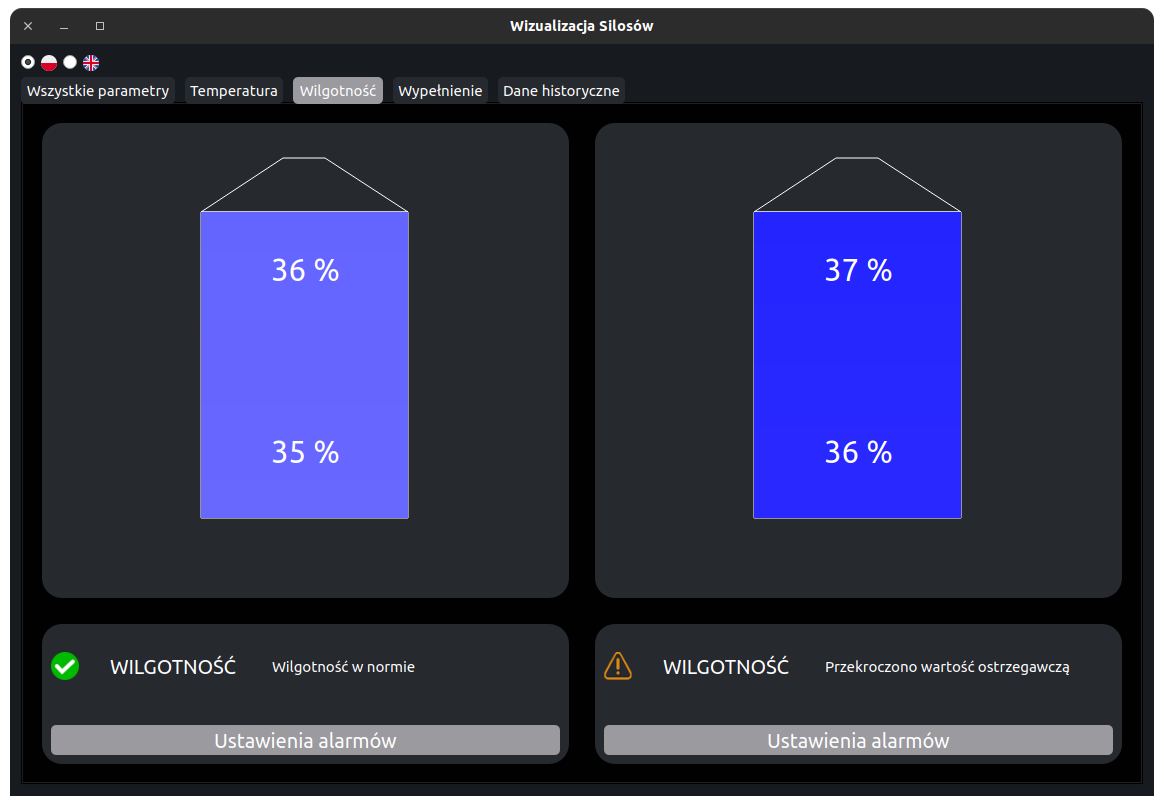
\includegraphics[width = \textwidth]{obrazy/hum_tab.png}
        \caption{Wygląd zakładki Wilgotność}
        \label{fig: hum tab}
    \end{figure}


    \begin{figure}[H]
        \centering
        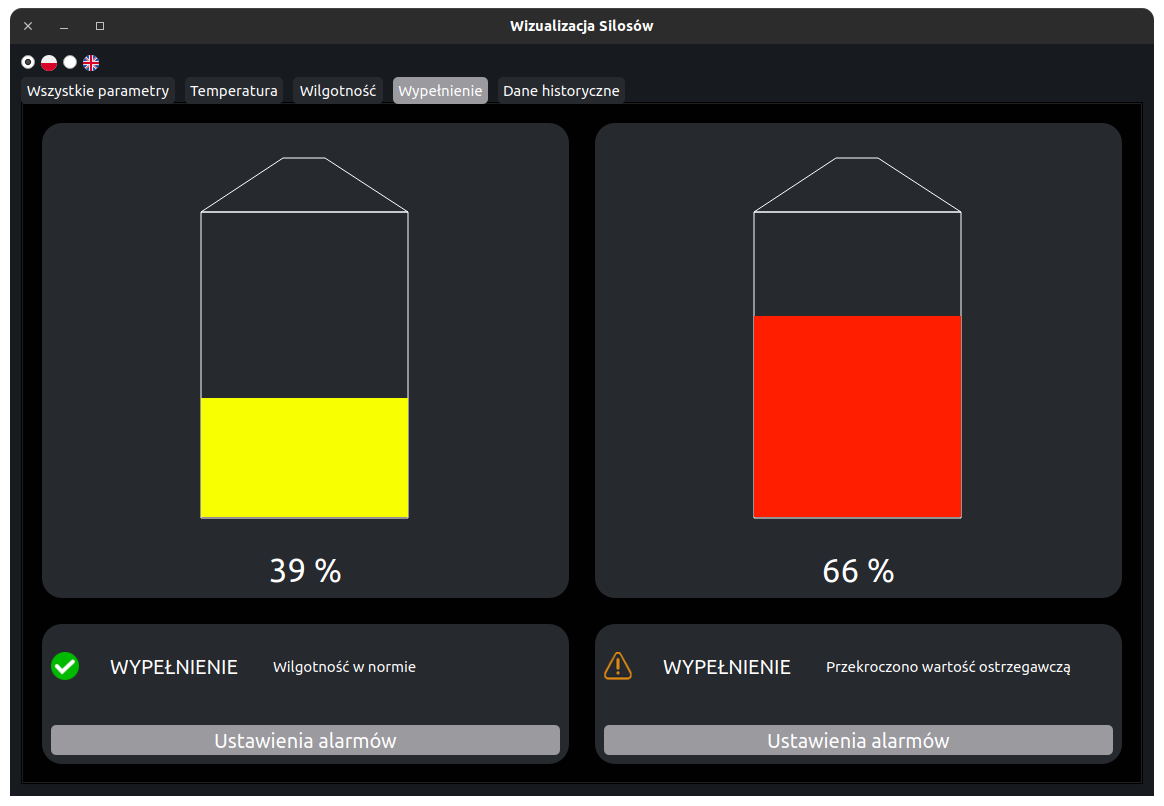
\includegraphics[width = \textwidth]{obrazy/temp_tab.png}
        \caption{Wygląd zakładki Wypełnienie}
        \label{fig: vol tab}
    \end{figure}


    \begin{figure}[H]
        \centering
        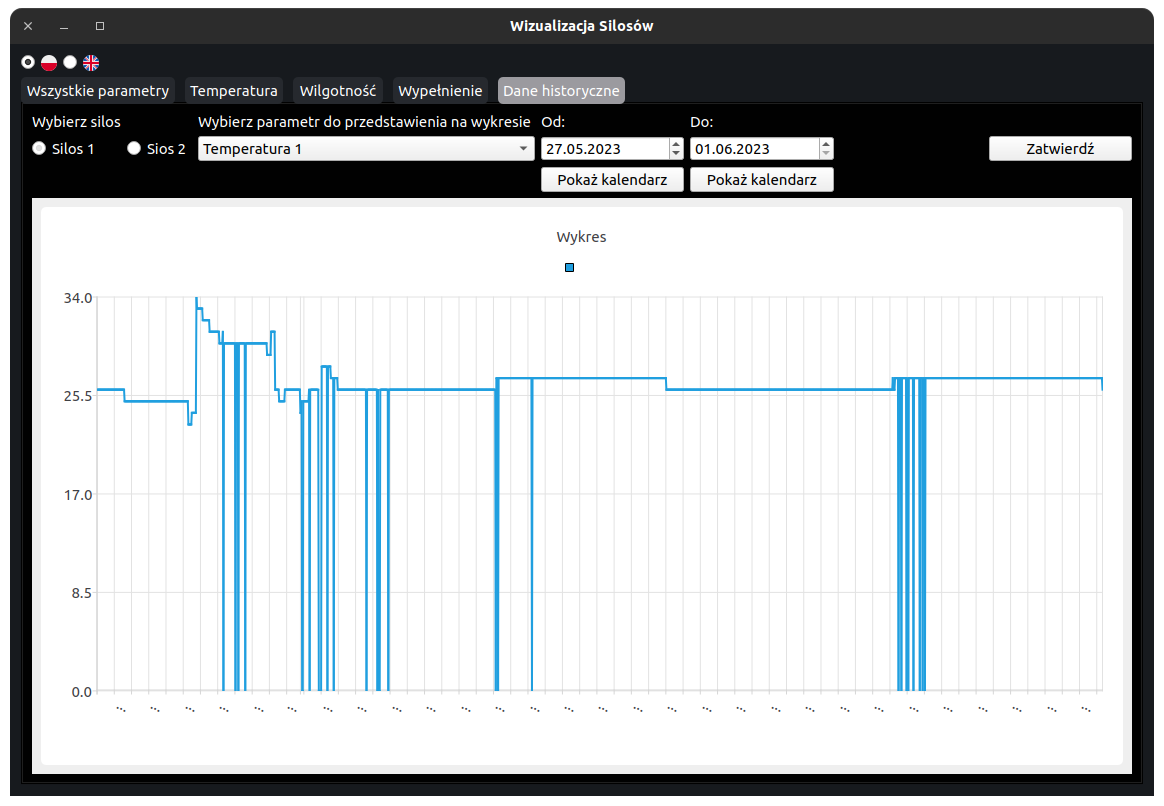
\includegraphics[width = \textwidth]{obrazy/hist_data_tab.png}
        \caption{Wygląd zakładki Dane Historyczne}
        \label{fig: hist data tab}
    \end{figure}


    \begin{figure}[H]
        \centering
        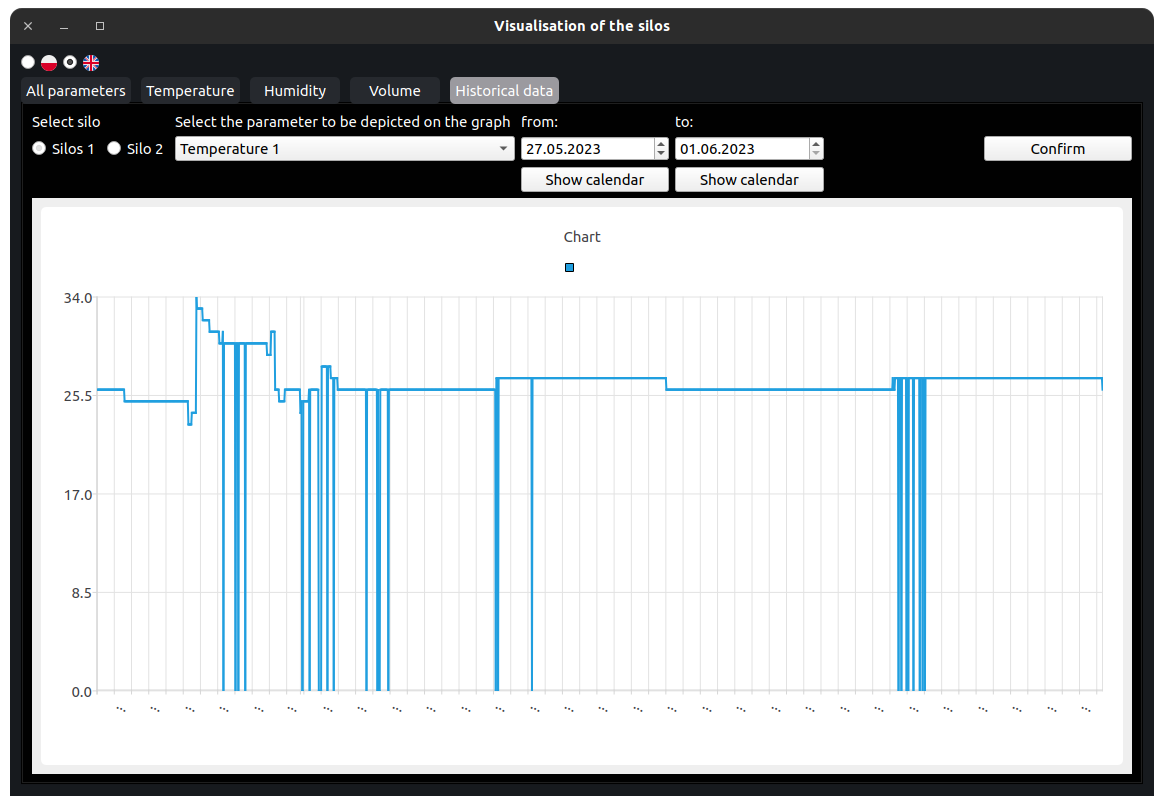
\includegraphics[width = \textwidth]{obrazy/ang.png}
        \caption{Zaprezentowanie tłumaczenia na ang}
        \label{fig: ang}
    \end{figure}


